\clearpage
\section{Anleitung Ladevorgang\label{sec:Anleitung_Laden}}
\responsible{Julia Stöger}
Während des Ladevorganges darf der Starttaster \textbf{nicht} gedrückt werden!
\begin{enumerate}
    \item Not-Aus--Schalter drücken
    \item Ladedeckel öffnen
    \item Ladegerät anschließen: Am Ladegerät werden die Zellenspannungen angezeigt.
    \begin{figure}[H]
        \centering
        \tcbox[top=-1pt,left=-1pt,right=-1pt,bottom=-1pt,colframe=black!70,colback=black!70]{\includegraphics[width=.3\textwidth]{Fotos/Ladegereat/DSC_8742_Ladegereat_Hauptanzeige.png}}
        \caption{Ladegerät Hauptanzeige \label{fig:Ladegeraet_Hauptanzeige}}
    \end{figure}
    \newpage
    \item Ladevorgang starten:
    \begin{enumerate}
        \item Die beiden mittleren Tasten des Ladegerätes drücken und die Option \glqq Dual Task \grqq\ auswählen.
        \begin{figure}[H]
            \centering
            \tcbox[top=-1pt,left=-1pt,right=-1pt,bottom=-1pt,colframe=black!70,colback=black!70]{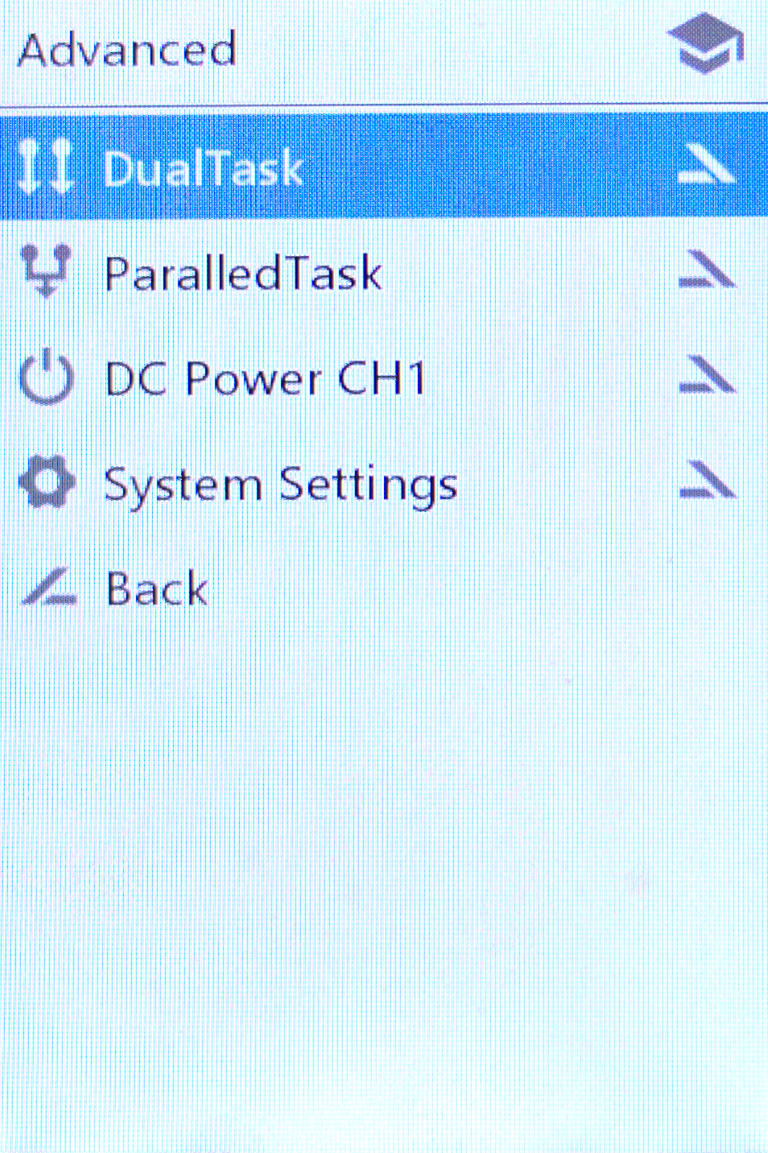
\includegraphics[width=.3\textwidth]{Fotos/Ladegereat/DSC_8744_Lademenue.png}}
            \caption{Ladegerät Task-Auswahl \label{fig:Ladegeraet_Menueanzeige}}
        \end{figure}
        \item Die Parameter wie in \autoref{fig:Ladegeraet_Menueanzeige2} einstellen und mit \glqq Start\grqq\ den Ladevorgang starten.
        % Mit den Touch-Buttons rechts oben oder unten lässt es sich durch das Menü         scrollen und somit die richtige Einstellung auswählen. 
        \begin{figure}[H]
            \centering
            \tcbox[top=-1pt,left=-1pt,right=-1pt,bottom=-1pt,colframe=black!70,colback=black!70]{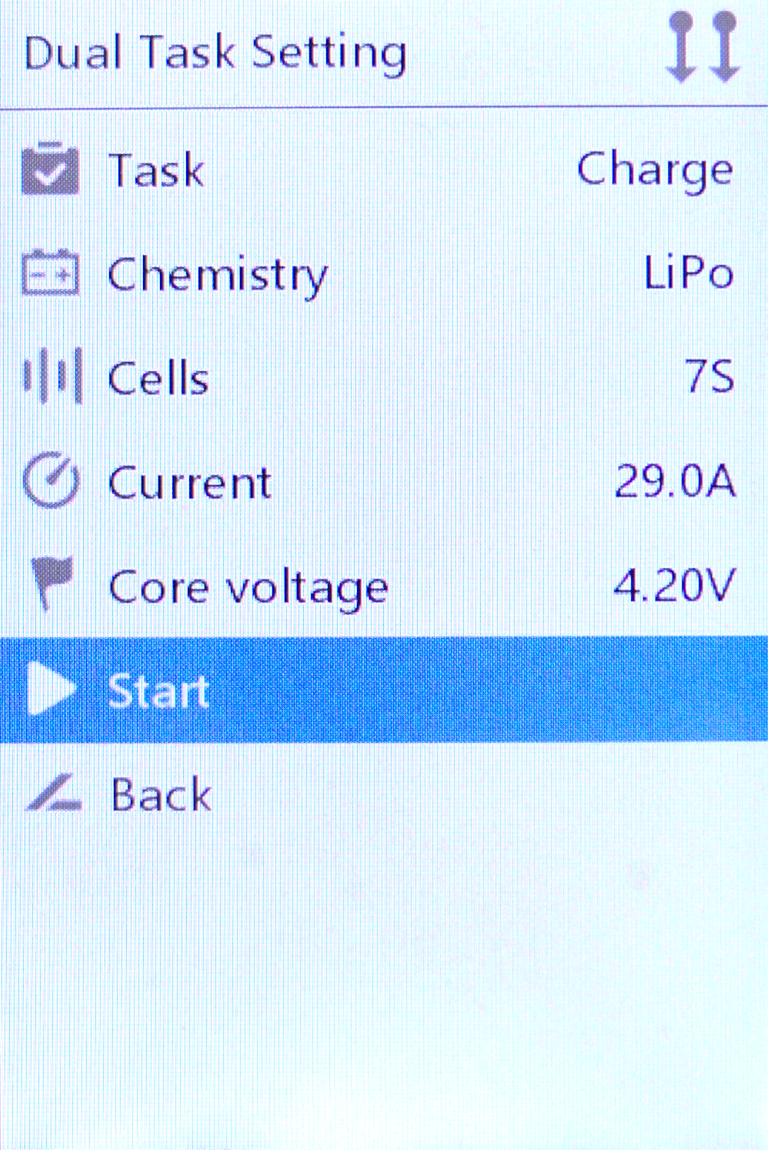
\includegraphics[width=.3\textwidth]{Fotos/Ladegereat/DSC_8745_Lademenue_2.png}}
            \caption{Ladegerät Einstellungen \label{fig:Ladegeraet_Menueanzeige2}}
        \end{figure}
    \end{enumerate}
    \newpage
    \item Während des Schnellladevorgangs leuchtet der obere Bereich des Displays orange -- siehe \autoref{fig:Ladegeraet_Ladezustand}
    \begin{figure}[H]
        \centering
        \tcbox[top=-1pt,left=-1pt,right=-1pt,bottom=-1pt,colframe=black!70,colback=black!70]{\includegraphics[width=.3\textwidth]{Fotos/Ladegereat/DSC_8747_Laden.png}}
        \caption{Ladegerät Schnellladevorgang \label{fig:Ladegeraet_Ladezustand}}
    \end{figure}
    \item Solbald der obere Bereich des Displays grün leuchtet, ist das Schnellladen abgeschlossen, aber der Ladevorgang ist noch nicht fertig.
    \item Erst wenn der obere Bereich des Displays blau leuchtet, ist der Ladevorgang abgeschlossen und kann mit Klicken auf die mittleren Touch-Buttons beendet werden
    \item Ladegerät abschließen \&\ Kabel in Ladebox verstauen
    \item Ladedeckel schließen
\end{enumerate}
